% !Mode:: "TeX:UTF-8"
% !TEX root = tjumain.tex

\iffalse
\bibliography{reference/reference.bib} % 欺骗latextools获取bib文件
\fi

%%%%%%% 正文 %%%%%%%

\chapter{引言}

笔者在学习高中数学时,无意间接触到了Taylor公式.对于这样一个可以用来逼近函数值的定理,笔者好奇其是否能在物理学中有所应用.本文记录了两个可以直接利用Taylor公式(方法)证明的命题,以及若干利用高阶无穷小、等价无穷小解决的问题.

由于笔者并没有正式地学习过物理学,本文中的纰漏在所难免.

\chapter{无穷小与Taylor公式}

\section{无穷小}

先介绍什么是无穷小、高阶无穷小、等价无穷小:

\begin{definition}
	在某一极限过程下,极限为$0$的函数称为\textbf{无穷小}.设无穷小$f(x)$和$g(x)~(x \to x_0)$且$g(x)$在$x_0$附近不为零,令$$\lim_{x \to x_0} \frac{f(x)}{g(x)}=a$$
	若$a=1$,则称$f(x)$和$g(x)$是\textbf{等价无穷小},记作$f(x) \sim g(x)$; \\
	若$a=0$,则称$f(x)$是$g(x)$的\textbf{高阶无穷小},(不严谨地)记作$f(x)=o(g(x))$.
\end{definition}

高阶无穷小、等价无穷小实际上描述的是一个“变化速率”的问题.例如,我们知道,在$0$附近$\sin x$的变化速率与$x$几乎是相同的,反映到具体数学语言上就是$$\lim_{x \to 0} \frac{\sin x}{x} = \lim_{x \to 0} \frac{(\sin x)'}{x'} = 1$$
	于是它们是等价无穷小. 

另外,在遇到几个不同阶的无穷小时,为了估计常常忽略更高阶的无穷小.例如$\Delta x+(\Delta x)^2$中可以忽略掉后项.


\section{Taylor公式及其证明}
\begin{theorem}{\textbf{带Peano余项的Taylor公式}\cite{ayumu}}
	设函数$f(x)$在$x_0$处有$n$阶导数,则当$x \to x_0$时,$$f(x) = f(x_0) + \frac{1}{1!}f'(x_0)(x-x_0) + \frac{1}{2!}f''(x_0)(x-x_0)^2 + \cdots + \frac{1}{n!}f^{(n)}(x_0)(x-x_0)^n + o[(x-x_0)^n]$$
\end{theorem}
\begin{proof}
	对$n$进行归纳证明:记$$T_{n}(f,x_0;x):=f(x_0) + \frac{1}{1!}f'(x_0)(x-x_0) + \frac{1}{2!}f''(x_0)(x-x_0)^2 + \cdots + \frac{1}{n!}f^{(n)}(x_0)(x-x_0)^n$$
	当$n=1$时,命题即为$$f(x)=f(x_0)+f'(x_0)(x-x_0)+o(x-x_0),~x \to x_0$$
	由无穷小增量公式,该命题成立; \\
	假设当$n=k$时命题成立.由于
	$$T_{k+1}(f,x_0;x)=f(x_0) + \frac{1}{1!}f'(x_0)(x-x_0) + \frac{1}{2!}f''(x_0)(x-x_0)^2 + \cdots + \frac{1}{(k+1)!}f^{(k+1)}(x_0)(x-x_0)^{k+1}$$
	故
	$$T'_{k+1}(f,x_0;x)=f'(x_0) + \frac{1}{1!}f''(x_0)(x-x_0) + \cdots + \frac{1}{k!}f^{(k+1)}(x_0)(x-x_0)^{k} = T_k(f',x_0;x)$$
	由l’Hôpital法则和归纳假设可知$$\lim_{x \to x_0} \frac{f(x)-T_{k+1}(f,x_0;x)}{(x-x_0)^{k+1}} = \frac{1}{k+1} \lim_{x \to x_0} \frac{f'(x)-T_{k}(f',x_0;x)}{(x-x_0)^{k}} = 0$$
	由归纳原理知原命题成立.
\end{proof}

可以认为,Taylor公式通过一个函数在某点附近的信息来估计函数值.更确切地说,它通过一个多项式拟合原函数.

在应用Taylor公式时,我们倾向于尽可能多地简化该式子.令$x_0=0$,即得到\textbf{Maclaurin公式}.

\begin{corollary}{\textbf{Maclaurin公式}}
	设函数$f(x)$在$0$处有$n$阶导数,则当$x \to 0$时,$$f(x)=f(0)+\frac{f'(0)}{1!}x + \frac{f''(0)}{2!}x^2 + \cdots + \frac{f^{(n)}(0)}{n!}x^n + o(x^n)$$
\end{corollary}

微元法中应用的“等价无穷小”本质上就是Maclaurin公式.因而在后文主要讨论的都是该公式的应用.


\chapter{Taylor公式(方法)的应用}

\section{推导变速直线运动公式}

先来看一个简单的结论.在匀变速直线运动中,位移关于时间的函数$x(t)$满足$$x(t) = x_0 + v_0t + \frac{1}{2}at^2$$
我们好奇能否将这个形式进行推广?如果知道物体在$0$时刻处的速度、加速度、加速度的变化率、加速度的变化率的变化率$\cdots$能否给出$x(t)$的表达式?

注意到,上式与Maclaurin公式的形式很像.若设$x(t)$表示在直线运动中从$0$时刻到$t$时刻中物体的位移量,这意味着$$x(t) = x(0) + \frac{1}{1!} x'(0)t + \frac{1}{2!} x''(0)t^2$$
然而这个形式不完全等价于Maclaurin公式,因为该公式的效用极限过程是$t \to 0$.换个思路,我们可以用接近于Taylor公式证明的方法来证明该加强命题:

\begin{proposition}{}
	设$a_i~(i=0,1,2,\cdots)$为常数,在$x(t)$的某一阶导函数为常值函数时,有$$x(t) = \sum_{i=0}^{\infty} a_ix^{(i)}(0) t^{i} = a_0x(0) + a_1x'(0)t + a_2x''(0)t^2 + \cdots$$
	其中$\{ a_n \}_{n=0}^{\infty}$满足$a_n = \dfrac{1}{n!}$.
\end{proposition}
\begin{remark}
	该命题的形式与Legendre定理类似.因为对任意$n>N$都有$x^{(n)}(0)=0$,故这是个有限项多项式.
\end{remark}
\begin{remark}
	若$x(t)$不存在任一阶导函数为常值函数,可以取某个足够大的$n$来近似计算.
\end{remark}
\begin{proof}
	设$x(t)$的第$n$阶导函数为常值函数,对$n$进行归纳证明.记$$T_n(x;t) := x(t) = x(0) + \frac{1}{1!} x'(0)t + \frac{1}{2!} x''(0)t^2 + \cdots + \frac{1}{n!} x^{(n)}(0)t^n$$
	$1^{\circ}~$当$n=1$时,由于此时物体作匀速直线运动,$x(t)=x(0)+x'(0)t$自然成立. \\
	$2^{\circ}~$假设$n=k$时命题成立.在$n=k+1$时,由于
	$$T_{k+1}(x;t) = x(0) + \frac{1}{1!} x'(0)t + \frac{1}{2!} x''(0)t^2 + \cdots + \frac{1}{(k+1)!} x^{(k+1)}(0)t^{k+1}$$
	$$T'_{k+1}(x;t) = x'(0) + \frac{1}{1!} x''(0)t + \frac{1}{2!} x'''(0)t^2 + \cdots + \frac{1}{k!} x^{(k+1)}(0)t^k = T_{k}(x';t)$$
	由归纳假设,$T_k(x',t)=x(t)$.故$x(t)=T_{k+1}(x;t)$. \\
	由数学归纳原理可知命题成立.
\end{proof}

命题3.1提供了一个有趣的直觉:如果能搞清楚某物体任一时间下的运动状态,我们就能推导它的运动全程.这个直觉被应用在了刘慈欣的科幻小说《镜子》\cite{liucixin}中:文中气象模拟员白冰通过对宇宙大爆炸时有限个物理量的控制模拟出了我们的宇宙.

\section{推导近地重力势能公式}

上一小节似乎是杀鸡用了牛刀.本小节更能体现出Taylor公式在处理近似时的重要作用.

\begin{proposition}
	在选取地表为零势能点时,近地物体的重力势能为$$E_{PG} \approx mgh$$
\end{proposition}
\begin{remark}
	当物体的质量到达天文质量级时,这个估计将会极不准确,因而只讨论物体质量远小于地球质量的情况.
\end{remark}

对于一个近地物体,设地球半径$R$,地表与该物体距离$h$,地球、该物体质量分别为$M,m$,$G$为万有引力常数,选择无穷远处为势能零点,则该物体的引力势能为(将其看做关于$h$的函数)$$E_P(h) = - \frac{GMm}{R+h}$$
由于$h \ll R$,令$h \to 0$,由Maclaurin公式,此时有
\begin{align*}
	E_P(h) &= E_P(0)+\frac{E'_P(0)}{1!}h + o(h^2) \\
	&\approx -\frac{GMm}{R} + \frac{GMm}{R^2} h
\end{align*}
由黄金代换公式,$$E_P(h) \approx -\frac{GMm}{R} + mgh$$
注意到这个式子的势能零点是无穷远处,而近地重力势能的势能零点是地表.这两个零势能点的势能差值等于地表处因(近似等价于)球心的万有引力而具有的势能(此时零势能点为无穷远处),这个值恰好为$$-\frac{GMm}{R}$$
于是近地处物体重力势能为(零势能点为地表)$$E_{PG} \approx mgh$$

\chapter{无穷小的应用}

\section{忽略高阶无穷小进行计算}

忽略高阶无穷小的方法以例题阐释:

\begin{example}
	如下$a-x$图所示,一物体作变加速度直线运动.已知其初速为$v_0$,加速度满足$a=a_0-kx$,求位移为$x_0$时物体的末速度$v_t$.
	\begin{figure}[htbp]
		\begin{center}
			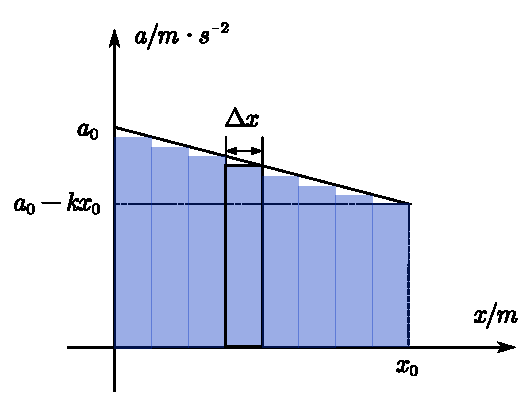
\includegraphics[width=7cm]{20230209.pdf}
		\end{center}
	\caption{}
	\end{figure}
\end{example}
\begin{solution}
	可以将$a-x$直线近似地看做数段折线,每一段折线长为$\Delta x$.观察其中某一段,设这一段加速度为$a$不变,那么这段折线与$x$轴围成的面积为$$S = a\Delta x = \frac{\Delta v}{\Delta t} \cdot \Delta x = v \cdot \Delta v$$
	其中,因为$$\Delta (v^2) = (v+\Delta v)^2 - v^2 = 2v \cdot \Delta v + (\Delta v)^2 = v \cdot \Delta v$$
	可知$$S = \frac{\Delta (v^2)}{2}$$
	将所有这样的矩形面积加在一起,就得到$$a_0x_0 - \frac{1}{2}kx_0^2 = \frac{v_t^2-v_0^2}{2}$$
	于是得到$$v_t = \sqrt{v_0^2 + a_0x_0 - \frac{1}{2}kx_0^2}$$
\end{solution}

不难发现,特别是在应用微元法时,可以通过忽略高阶无穷小简化计算.

\section{通过等价无穷小近似计算}

由Maclaurin公式,可以得到一些常见函数在$x \to 0$时的展开式:

\begin{proposition}
	当$x \to 0$时,
	$$\sin x = x - \frac{x^3}{3!} + \frac{x^5}{5!} - \frac{x^7}{7!} + \cdots + \frac{(-1)^{k-1}x^{2k-1}}{(2k-1)!} + o(x^{2k-1})$$
	$$\cos x = 1 - \frac{x^2}{2!} + \frac{x^4}{4!} - \frac{x^6}{6!} + \cdots + \frac{(-1)^{k}x^{2k}}{(2k)!} + o(x^{2k})$$
	$$(1+x)^{\alpha} = 1 + \alpha x + \frac{\alpha (\alpha -1)}{2!}x^2 + \cdots + \frac{\alpha (\alpha -1) \cdots (\alpha -n+1)}{n!} x^n + o(x^n)$$
\end{proposition}

忽略高阶无穷小,得到以下重要的等价无穷小:

\begin{proposition}
	当$x \to 0$时, 
	$$(1+x)^{\alpha} -1 \sim \alpha x, \qquad \sin x \sim x \sim\tan x, \qquad 1-\cos x \sim \dfrac{x^2}{2}$$
\end{proposition}
\begin{remark}
	虽然$\tan x$的展开式不能用初等方法表达,直接利用定义,我们仍可以证明它与$x$是等价无穷小.
\end{remark}

上述等价无穷小会给计算带来很多方便.

\begin{example}
	如图i所示,岸上一小人以恒定速度$v$拉动绳子的一头,船上的小人抓住绳子的另一头,求船速$v'$.
	\begin{figure}[htbp]
		\begin{center}
			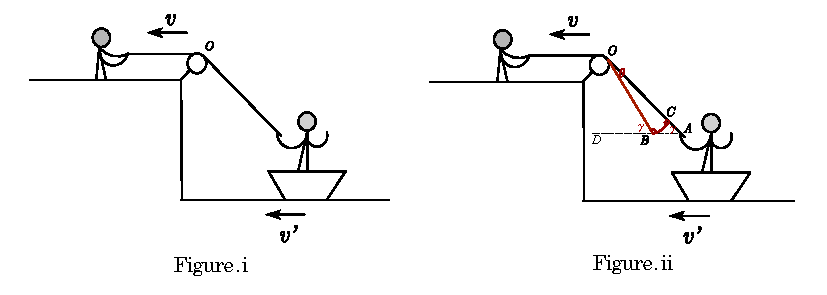
\includegraphics[width=14cm]{4.1.pdf}
		\end{center}
	\caption{}
	\end{figure}
\end{example}
\begin{solution}
	如图ii所示,在一段极短的时间$\Delta t$内,设绳子的一头从$A$移动到$B$,过点$B$作$BC \bot OB$. \\
	在$\vartriangle OBC$中,由于$\tan \theta \sim \sin \theta$,又$BC = \tan \theta OB = \sin \theta OC$,故可看做$OC=OB=l$,此时$\angle OBC = 90^{\circ}$.同理可知$\angle OCB = 90^{\circ}$.于是$\overset{\LARGE{\frown}}{BC} = \theta l = \tan \theta l = BC$,可将$\overset{\LARGE{\frown}}{BC}$看做直线. \\
	考虑$\angle OBD=\gamma$,于是$\angle CBA=90^{\circ} - \gamma$,那么$\angle CAB = \gamma$.在直角三角形$\vartriangle ABC$中,$AB = v' \Delta t$,$AC = v \Delta t$,故$v \Delta t = \cos \gamma v' \Delta t$,解得$v' = \dfrac{v}{\cos \gamma}$.
\end{solution}

\begin{example} \cite{xnlljbsi}
	一块厚度为$h$的匀质长方形物块,静止地放在半径为$R$的半圆柱顶面上,如图i所示.设摩擦系数足够大,长方体物块与柱面不发生滑动.求此静止位置为稳定平衡的条件. \\
	注:物体平衡位置为稳定平衡位置的条件是:当此物体稍微偏离平衡位置时,将受到指向平衡位置的合力作用(平衡力),使物体回到平衡位置.
	
	\begin{figure}[htbp]
		\begin{center}
			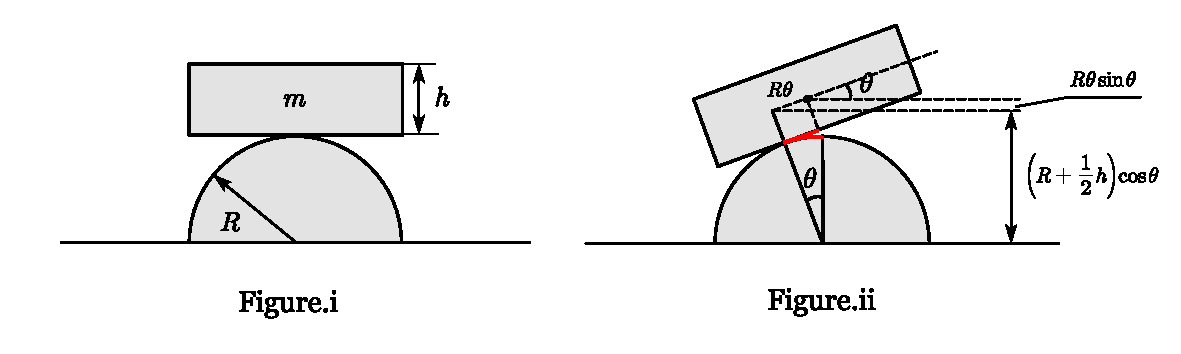
\includegraphics[width=14cm]{202302092.pdf}
		\end{center}
	\caption{}
	\end{figure}
\end{example}
\begin{solution}
	从势能的角度看,在物块旋转一个微小角度之后,为了保证其受到向上的某个力,需要让重力势能增加.也就是说,要让旋转之后的重心高度大于原重心高度. \\
	如图ii所示,在物块滚动一个极小的角度$\theta$后,由于红色线段与红色弧线长度相等(由滚动的定义),可以得到旋转后重心的高度$y$:
	$$y = (R+ \frac{h}{2})\cos \theta + R\theta \sin \theta$$
	因为$y$大于原重心高度$R + \dfrac{h}{2}$,可以列出$$(R+ \frac{h}{2})\cos \theta + R\theta \sin \theta - R - \frac{h}{2} > 0$$
	$$(R+ \frac{h}{2})(1-\frac{\theta ^2}{2}) + R\theta ^2 - R - \frac{h}{2} > 0$$
	解得$R>\dfrac{h}{2}$.
\end{solution}





%%%%%%% 结论 %%%%%%%

\addcontentsline{toc}{chapter}{结\quad 论} %添加到目录中

\chapter*{结\quad 论}

泰勒公式与无穷小都提供了一种重要的思想:忽略一些相对较小的量进而进行近似计算,这在大多数时候都不追求精确解析解的物理学中尤为重要.
